\documentclass[aspectratio=169,11pt]{beamer}
\usepackage[T1]{fontenc}
\usepackage{lmodern,amsmath,amssymb,mathtools,bm,booktabs,array,graphicx,tikz}
\usetikzlibrary{arrows.meta,positioning,calc,decorations.pathreplacing,patterns}
\definecolor{ink}{HTML}{17344D}\definecolor{accent}{HTML}{087E8B}\definecolor{pale}{HTML}{EDF5F5}\definecolor{gold}{HTML}{AD6B19}
\providecommand{\dd}{\,\mathrm{d}}\providecommand{\R}{\mathbb{R}}
\providecommand{\E}{\mathbb{E}}\providecommand{\Var}{\operatorname{Var}}
\providecommand{\Cov}{\operatorname{Cov}}\providecommand{\diag}{\operatorname{diag}}
\providecommand{\norm}[1]{\left\lVert#1\right\rVert}
\providecommand{\abs}[1]{\left|#1\right|}
\usefonttheme{professionalfonts}
\setbeamercolor{normal text}{fg=black,bg=white}
\setbeamercolor{frametitle}{fg=ink,bg=white}
\setbeamercolor{title}{fg=ink}\setbeamercolor{structure}{fg=accent}
\setbeamercolor{block title}{fg=ink,bg=pale}\setbeamercolor{block body}{fg=black,bg=pale!40}
\setbeamercolor{alerted text}{fg=accent}
\setbeamerfont{frametitle}{size=\Large,series=\bfseries}
\setbeamerfont{title}{size=\LARGE,series=\bfseries}
\setbeamertemplate{navigation symbols}{}
\setbeamersize{text margin left=.7cm,text margin right=.7cm}
\setbeamertemplate{frametitle}{\vspace{.18cm}\insertframetitle\par\vspace{.1cm}{\color{accent}\hrule height .6pt}\vspace{.12cm}}
\newcommand{\notestarget}{notes.pdf}\newcommand{\noteslabel}{Notes}
\setbeamertemplate{footline}{\hspace{.7cm}\color{ink}\scriptsize Mathematical Modeling\quad\href{\notestarget}{\noteslabel}\hfill\insertframenumber\,/\,\inserttotalframenumber\hspace{.7cm}\vspace{.18cm}}
\setbeamercovered{invisible}
\hypersetup{pdfauthor={Zan Ahmad},pdftitle={Membrane currents and Hodgkin--Huxley gate kinetics},pdfpagemode=UseNone}
\begin{document}
\begin{frame}[plain]\vfill
{\small\color{accent} Mathematical Modeling \quad Lecture 9}\par\medskip
{\raggedright\hyphenpenalty=10000\exhyphenpenalty=10000\LARGE\bfseries\color{ink} Membrane currents and Hodgkin--Huxley gate kinetics}\par\bigskip
Zan Ahmad\par\smallskip
{\small Fall 2024}\par\vfill\end{frame}
\renewcommand{\notestarget}{notes.pdf\#note-membrane-capacitance-and-the-sign-of-current}
\begin{frame}[t,fragile,label=slide-membrane-charge-balance]{Membrane charge balance}
\[V=\phi_{\mathrm{in}}-\phi_{\mathrm{out}},\qquad C\dot V=I_{\mathrm{app}}-I_{\mathrm{ion}}.\]\pause{} Applied current is positive inward; ionic current is positive outward.
\end{frame}
\renewcommand{\notestarget}{notes.pdf\#note-membrane-capacitance-and-the-sign-of-current}
\begin{frame}[t,fragile,label=slide-density-and-total-current]{Density and total current}
\[[C]=\mu\mathrm F/\mathrm{cm}^2,\quad [V]=\mathrm{mV},\quad[t]=\mathrm{ms}.\]\pause{}\[\mu\mathrm F\cdot\mathrm{mV}/\mathrm{ms}=\mu\mathrm A,\qquad I_{\mathrm{total}}=A_mI_{\mathrm{density}}.\]
\end{frame}
\renewcommand{\notestarget}{notes.pdf\#note-conductance-reversal-potential-and-channel-gates}
\begin{frame}[t,fragile,label=slide-conductance-and-electrochemical-driving-difference]{Conductance and electrochemical driving difference}
\[I_j=g_j(V-E_j).\]\pause{} A reversal potential makes one current zero, not necessarily the total current.\par\medskip At $V<E_j$, this outward-positive current is negative.
\end{frame}
\renewcommand{\notestarget}{notes.pdf\#note-conductance-reversal-potential-and-channel-gates}
\begin{frame}[t,fragile,label=slide-the-three-conductance-laws]{The three conductance laws}
\[g_{\mathrm{Na}}=120m^3h,\quad g_{\mathrm K}=36n^4,\quad g_{\mathrm L}=0.3.\]\pause{}\[(E_{\mathrm{Na}},E_{\mathrm K},E_{\mathrm L})=(45,-82,-59)\,\mathrm{mV}.\] Conductances are in $\mathrm{mS}/\mathrm{cm}^2$.
\end{frame}
\renewcommand{\notestarget}{notes.pdf\#note-gate-kinetics-and-the-voltage-clamp-solution}
\begin{frame}[t,fragile,label=slide-gate-opening-and-closing]{Gate opening and closing}
\[\dot s=\alpha_s(V)(1-s)-\beta_s(V)s,\qquad s\in\{m,h,n\}.\]\pause{} The source fractions enforce availability; rates are nonnegative and measured per millisecond.
\end{frame}
\renewcommand{\notestarget}{notes.pdf\#note-gate-kinetics-and-the-voltage-clamp-solution}
\begin{frame}[label=slide-voltage-clamp-relaxation-figure]{Voltage-clamp relaxation}
\centering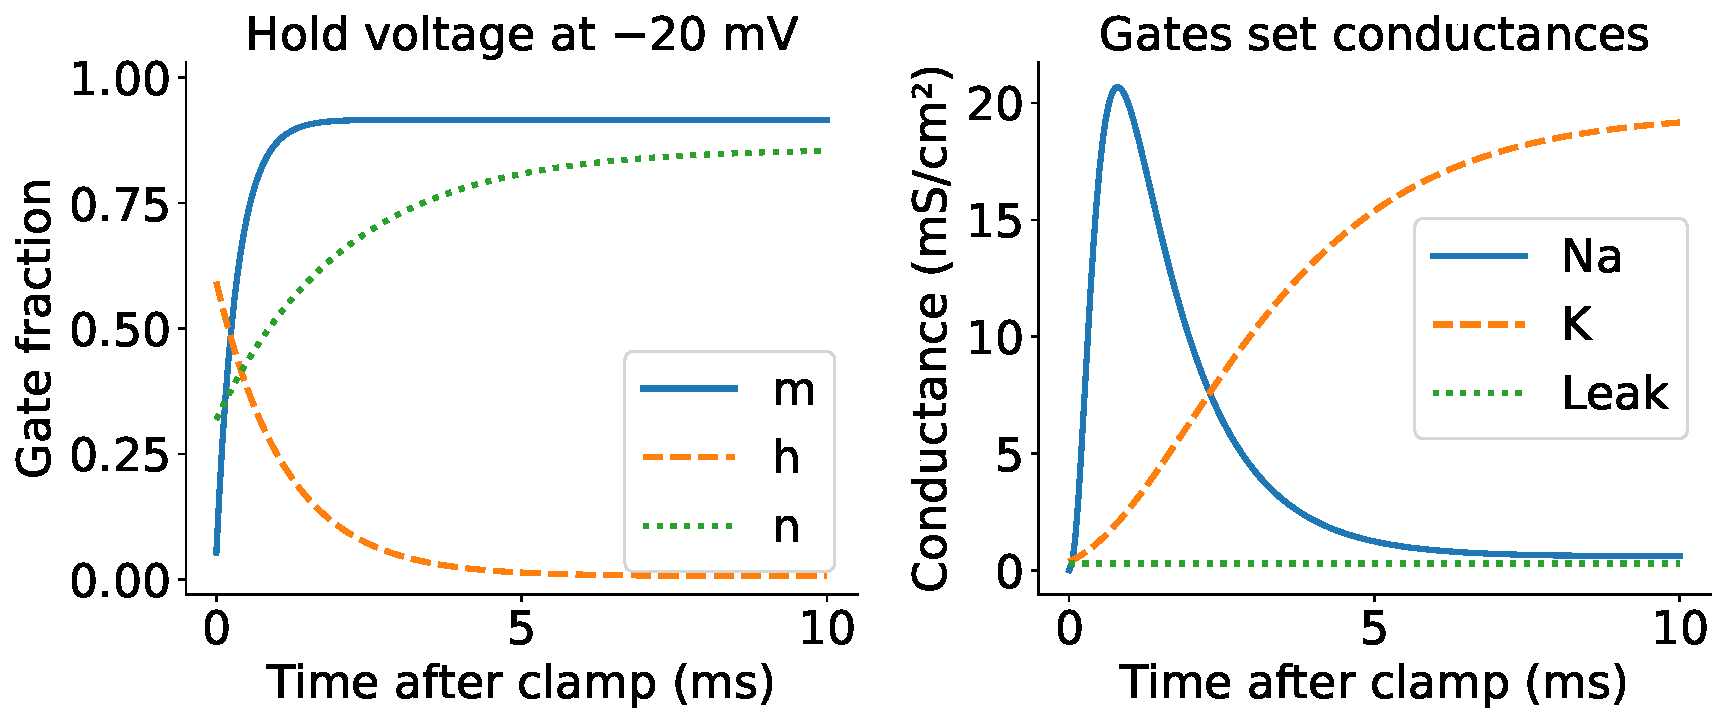
\includegraphics[width=.98\linewidth,height=.69\textheight,keepaspectratio]{voltage-clamp.pdf}\end{frame}
\renewcommand{\notestarget}{notes.pdf\#note-gate-kinetics-and-the-voltage-clamp-solution}
\begin{frame}[t,fragile,label=slide-voltage-clamp-relaxation]{Voltage-clamp relaxation}
\[s_\infty=\frac\alpha{\alpha+\beta},\quad\tau_s=\frac1{\alpha+\beta}.\]\pause{}\[s(t)=s_\infty+(s_0-s_\infty)e^{-t/\tau_s}.\]
\end{frame}
\renewcommand{\notestarget}{notes.pdf\#note-gate-kinetics-and-the-voltage-clamp-solution}
\begin{frame}[t,fragile,label=slide-a-constant-rate-gate-calculation]{A constant-rate gate calculation}
$\alpha=0.2$, $\beta=0.8\,\mathrm{ms}^{-1}$, $s_0=0.9$:\[s_\infty=0.2,\quad\tau_s=1\,\mathrm{ms},\quad s(3)=0.2+0.7e^{-3}\simeq0.23485.\]
\end{frame}
\renewcommand{\notestarget}{notes.pdf\#note-rate-functions-and-removable-singularities}
\begin{frame}[t,fragile,label=slide-activation-rate-functions]{Activation rate functions}
\[F(z)=\frac z{1-e^{-z}},\quad F(0)=1.\]\pause{}\[\begin{aligned}\alpha_m&=F((V+45)/10),&\beta_m&=4e^{-(V+70)/18},\\\alpha_n&=0.1F((V+60)/10),&\beta_n&=0.125e^{-(V+70)/80}.\end{aligned}\]
\end{frame}
\renewcommand{\notestarget}{notes.pdf\#note-rate-functions-and-removable-singularities}
\begin{frame}[t,fragile,label=slide-sodium-availability-rates]{Sodium availability rates}
\[\alpha_h=0.07e^{-(V+70)/20},\qquad\beta_h=\frac1{1+e^{-(V+40)/10}}.\]\pause{} $h$ is a gate variable, not the numerical time step.\par\medskip Its loss during depolarization helps terminate sodium conduction.
\end{frame}
\renewcommand{\notestarget}{notes.pdf\#note-rate-functions-and-removable-singularities}
\begin{frame}[t,fragile,label=slide-stable-evaluation-near-a-removable-singularity]{Stable evaluation near a removable singularity}
\[F(z)=1+\frac z2+\frac{z^2}{12}-\frac{z^4}{720}+O(z^6).\]\pause{} Use a local series near zero and $-\operatorname{expm1}(-z)$ elsewhere.\par\medskip The physical rate remains finite at $V=-45,-60\,\mathrm{mV}$.
\end{frame}
\renewcommand{\notestarget}{notes.pdf\#note-rest-feedback-and-the-pulse-experiment}
\begin{frame}[t,fragile,label=slide-a-self-consistent-resting-state]{A self-consistent resting state}
\[s=s_\infty(V_*),\qquad I_{\mathrm{ion}}(V_*,s_\infty(V_*))=0.\]\pause{} The current parameter set gives $V_*\simeq-69.89767\,\mathrm{mV}$.
\end{frame}
\renewcommand{\notestarget}{notes.pdf\#note-rest-feedback-and-the-pulse-experiment}
\begin{frame}[t,fragile,label=slide-regenerative-and-terminating-feedback]{Regenerative and terminating feedback}
Depolarization increases sodium activation, which can increase inward current.\pause{}\par\medskip Sodium availability then falls; potassium conductance rises; driving differences also change.\par\medskip Current is conductance times driving difference.
\end{frame}
\renewcommand{\notestarget}{notes.pdf\#note-rest-feedback-and-the-pulse-experiment}
\begin{frame}[label=slide-current-driven-pulse-experiments-figure]{Current-driven pulse experiments}
\centering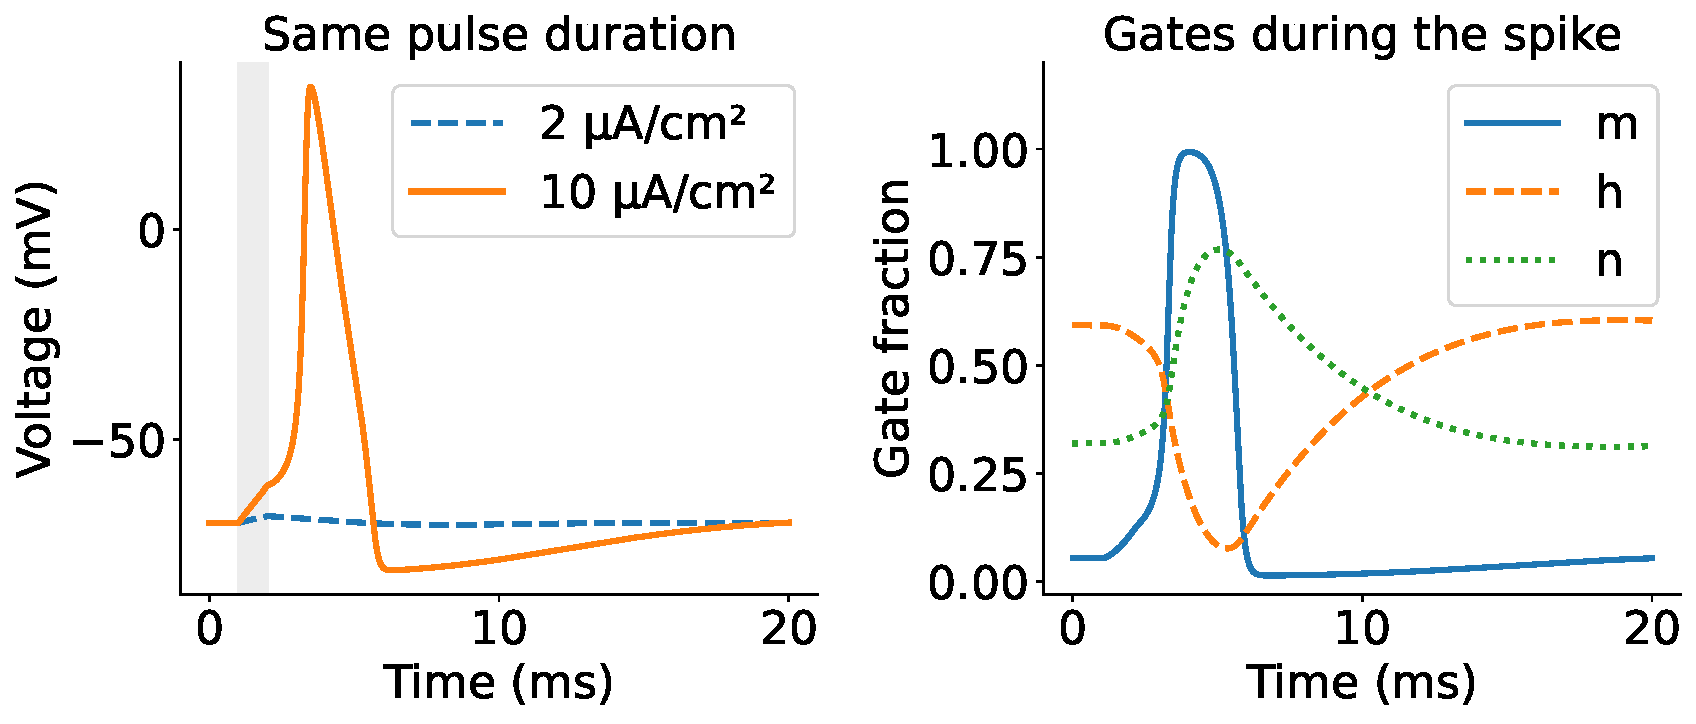
\includegraphics[width=.98\linewidth,height=.69\textheight,keepaspectratio]{pulse-and-gates.pdf}\end{frame}
\renewcommand{\notestarget}{notes.pdf\#note-rest-feedback-and-the-pulse-experiment}
\begin{frame}[t,fragile,label=slide-current-driven-pulse-experiments]{Current-driven pulse experiments}
Pulse interval: $[1,2)\,\mathrm{ms}$.\par Amplitudes: $2$ and $10\,\mu\mathrm A/\mathrm{cm}^2$.\pause{}\par\medskip A small excursion and a spike are two specified experiments, not a universal threshold measurement.
\end{frame}
\renewcommand{\notestarget}{notes.pdf\#note-a-signed-current-calculation}
\begin{frame}[t,fragile,label=slide-a-signed-ionic-current-sum]{A signed ionic-current sum}
At $V=-60\,\mathrm{mV}$, prescribe $g=(0.12,0.36,0.30)$:\[I_{\mathrm{Na}}=-12.6,\quad I_{\mathrm K}=7.92,\quad I_{\mathrm L}=-0.30.\]\pause{}\[I_{\mathrm{ion}}=-4.98\,\mu\mathrm A/\mathrm{cm}^2.\]
\end{frame}
\renewcommand{\notestarget}{notes.pdf\#note-a-signed-current-calculation}
\begin{frame}[t,fragile,label=slide-the-voltage-increment-from-current-balance]{The voltage increment from current balance}
\[\dot V=\frac{2-(-4.98)}1=6.98\,\mathrm{mV/ms}.\]\pause{}\[\Delta V\simeq0.05(6.98)=0.349\,\mathrm{mV},\qquad V^+\simeq-59.651\,\mathrm{mV}.\]
\end{frame}
\renewcommand{\notestarget}{notes.pdf\#note-gate-preserving-integration-of-the-coupled-system}
\begin{frame}[t,fragile,label=slide-an-exact-gate-substep]{An exact gate substep}
Freeze $V=V^k$ during $\Delta t$:\[s^{k+1}=s_\infty(V^k)+[s^k-s_\infty(V^k)]e^{-\Delta t/\tau_s(V^k)}.\]\pause{} This is a convex combination; no clipping is needed.
\end{frame}
\renewcommand{\notestarget}{notes.pdf\#note-gate-preserving-integration-of-the-coupled-system}
\begin{frame}[t,fragile,label=slide-an-exact-frozen-conductance-voltage-substep]{An exact frozen-conductance voltage substep}
\[G=\sum_jg_j,\quad V_{\mathrm{tar}}=\frac{I_{\mathrm{app}}+\sum_jg_jE_j}{G}.\]\pause{}\[V^{k+1}=V_{\mathrm{tar}}+(V^k-V_{\mathrm{tar}})e^{-G\Delta t/C}.\]
\end{frame}
\renewcommand{\notestarget}{notes.pdf\#note-gate-preserving-integration-of-the-coupled-system}
\begin{frame}[t,fragile,label=slide-event-alignment-and-delivered-charge]{Event alignment and delivered charge}
\[\int I_{\mathrm{app}}\,\dd t=10\,\mu\mathrm A\,\mathrm{ms}/\mathrm{cm}^2\] for the $10$-unit, one-millisecond pulse.\pause{}\par\medskip End a time step at each pulse edge; otherwise refinement can change the input itself.
\end{frame}
\renewcommand{\notestarget}{notes.pdf\#note-gate-preserving-integration-of-the-coupled-system}
\begin{frame}[t,fragile,label=slide-accuracy-of-the-coupled-membrane-calculation]{Accuracy of the coupled membrane calculation}
Exact substeps do not imply an exact coupled solution.\pause{}\par\medskip Check rest, gate bounds, rate limits, and common-time refinement.\par\medskip The sequential split is generally first order in the full state; voltage alone may show higher apparent order in a specific experiment.
\end{frame}
\end{document}
